\documentclass{standalone}
\usepackage{mathpazo}
\usepackage[american]{circuitikz}

\begin{document}
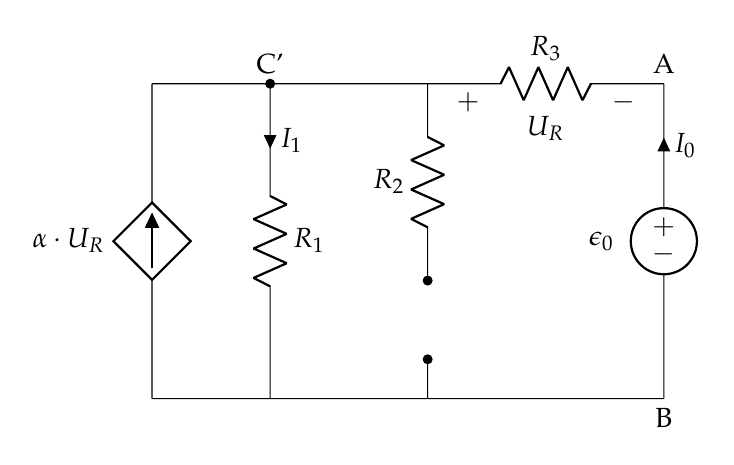
\begin{tikzpicture}
  \coordinate (A) at (0,0);
  \coordinate (B) at ($(A) + (1.5, 0)$) ;
  \coordinate (C) at ($(B) + (2, 0)$) ;
  \coordinate (D) at ($(C) + (3, 0)$) ;
  \coordinate (E) at ($(A) + (0, 4)$) ;
  \coordinate (F) at ($(B) + (0, 4)$) ;
  \coordinate (G) at ($(C) + (0, 4)$) ;
  \coordinate (H) at ($(D) + (0, 4)$) ;
  \draw
  (A) to [cI, l=$\alpha \cdot U_R$] (E)
  (B) to [R, l_ = $R_1$, -*, i_< = $I_1$] (F) node[above] {C'}
  (C) to [short,-*] ++(0,0.5)
  (G) to [short] ++(0,-0.5)
  to [R, l_ = $R_2$] ++(0,-1.5)
  to [short,-*] ++(0,-0.5)
  (G) to [R, l = $R_3$, -, v = $U_R$] (H) node[above] {A}
  (A) to [short, -] (D) node[below] {B}
  (E) to [short] (G)
  (H) to [V, v_=$\epsilon_0$, i = $I_0$] (D);
\end{tikzpicture}
\end{document}